\documentclass[11pt,titlepage]{article}
\usepackage[reqno]{amsmath}
\usepackage{amssymb}
\usepackage{epsf}
\usepackage{url}

% === additional commands/packages/settings ===
\usepackage{graphicx,psfrag,natbib}
\usepackage{setspace}
\usepackage{vmargin}
\setpapersize{USletter}
% \addtolength{\oddsidemargin}{-.55in}
% \addtolength{\evensidemargin}{-.55in}
% \addtolength{\textwidth}{1.1in}
% \addtolength{\textheight}{.9in}
% %\addtolength{\topmargin}{-.6in}
% \addtolength{\topmargin}{-.1in}

% === dcolumn package ===
\usepackage{dcolumn}
\newcolumntype{.}{D{.}{.}{-1}}
\newcolumntype{d}[1]{D{.}{.}{#1}}

% === newcommands from sei.tex ===
\newcommand{\EI}{\ensuremath{{\mathfrak EI}}}
\newcommand{\Tiny}{\tiny}
\newcommand{\sump}{\sum_{i=1}^p}
\newcommand{\mean}{\frac{1}{p}\sump}
\newcommand{\ub}{\Dot{\beta}}
\newcommand{\ut}{\Dot{\theta}}
\newcommand{\bbeta}{{\mathfrak B}}
\newcommand{\btheta}{{\mathfrak T}}
\newcommand{\blambda}{{\mathfrak L}}
\newcommand{\bbetau}{\breve{\mathfrak B}}
\newcommand{\bV}{{\cal V}}
\newcommand{\sigmau}{\breve{\sigma}}
\newcommand{\Sigmau}{\breve{\Sigma}}
\newcommand{\rhou}{\breve{\rho}}
\newcommand{\psiu}{\breve{\psi}}
\newcommand{\Eu}{\breve{\text{E}}}
\newcommand{\Vu}{\breve{\text{V}}}
\newcommand{\Bb}{B^b}
\newcommand{\Bw}{B^w}
\newcommand{\NbD}{{N_i^{bD}}}
\newcommand{\NwD}{{N_i^{wD}}}
\newcommand{\NbR}{{N_i^{bR}}}
\newcommand{\NwR}{{N_i^{wR}}}
\newcommand{\NbN}{{N_i^{bN}}}
\newcommand{\NwN}{{N_i^{wN}}}
\newcommand{\tp}{{\mbox{\Tiny{+}}}}
\newcommand{\NpD}{{N_i^D}}
\newcommand{\NpR}{{N_i^{R}}}
\newcommand{\NpN}{{N_i^{N}}}
\newcommand{\Nbp}{{N_i^{b}}}
\newcommand{\Nwp}{{N_i^{w}}}
\newcommand{\Npp}{{N_i}}
\newcommand{\Nppp}{{N}}
\newcommand{\Nbpp}{{N^{b}}}
\newcommand{\Nwpp}{{N^{w}}}
\newcommand{\sumpN}{\sump\Npp}
\newcommand{\NsumpN}{\frac{1}{\Nppp}\sumpN}
\newcommand{\nbp}{{N_i^{bT}}}
\newcommand{\nwp}{{N_i^{wT}}}
\newcommand{\npp}{{N_i^{T}}}
\newcommand{\NbV}{{N_i^{bT}}}
\newcommand{\NwV}{{N_i^{wT}}}
\newcommand{\NpV}{{N_i^{T}}}
\newcommand{\xb}{\bar{X}}
\newcommand{\wb}{\bar{W}}
\newcommand{\tb}{\bar{T}}
\newcommand{\cx}{{\mathbb X}}
\newcommand{\cw}{{\mathbb W}}
\newcommand{\ct}{{\mathbb T}}
\newcommand{\cpij}{{\mathbb P}^*_{ij}}
\newcommand{\cpi}{{\mathbb P}^*_i}
\newcommand{\cwd}{{\dot{\mathbb W}}}
\newcommand{\ctd}{{\dot{\mathbb T}}}
\newcommand{\cxd}{{\dot{\mathbb X}}}
\newcommand{\cxb}{\bar{\mathbb X}}
\newcommand{\cz}{{\mathbb G}}
\newcommand{\ch}{{\mathbb H}}
\newcommand{\cm}{{\mathbb M}}
\newcommand{\E}{{\textbf{E}}}
\newcommand{\V}{{\textbf{V}}}
\newcommand{\C}{{\textbf{C}}}
\newcommand{\rE}{{\text{E}}}
\newcommand{\rV}{{\text{V}}}
\newcommand{\rC}{{\text{C}}}
\newcommand{\TN}{\text{TN}}
\newcommand{\BN}{\text{BN}}
\newcommand{\N}{\text{N}}
\renewcommand{\P}{\text{P}}
\newcommand{\D}{\textbf{D}}
\newcommand{\R}{\ensuremath{\textbf{R}}}
\newcommand{\Rr}{\ensuremath{\{\textbf{R}\diagdown r}\}}
\newcommand{\bC}{\ensuremath{\textbf{C}}}
\newcommand{\Cc}{\ensuremath{\{\textbf{C}\diagdown c}\}}
\newcommand{\one}{{\mathbf{1}}}
\newcommand{\Q}{\ensuremath{\overset{\vspace{3em}}{\text{\Huge ?}}}}
\newlength{\padsp}
\settowidth{\padsp}{$(\beta^w_i=\nwp/\Nwp)$}
\newcommand{\padbw}{\hspace*\padsp}
\newcommand{\bkappa}{\boldsymbol{\kappa}}

\newcommand{\bb}{\beta^{\text{bad}}}
\newcommand{\bg}{\beta^{\text{good}}}

\title{Did Illegally Counted Absentee Ballots Decide the 2000 U.S.\ 
  Presidential Election?}

\author{Kosuke Imai\thanks{Ph.D. candidate, Department of Government,
    Harvard University. (Center for Basic Research in the Social
    Sciences, 34 Kirkland, Cambridge MA 02138;
    \texttt{http://www.people.fas.harvard.edu/\~kimai},
    \texttt{KImai@Fas.Harvard.Edu}}
\and %
Gary King\thanks{Professor of Government, Harvard University and
  Senior Science Advisor, Evidence and Information for Policy Cluster,
  World Health Organization (Center for Basic Research in the Social
  Sciences, 34 Kirkland Street, Harvard University, Cambridge MA
  02138; \texttt{http://GKing.Harvard.Edu}, \texttt{King@Harvard.Edu},
  (617) 495-2027).}  }

\begin{document}
\maketitle

\begin{abstract}
  Although it was not widely known until much later, Al Gore received
  202 more votes than George W.\ Bush on election day in Florida.
  George W.\ Bush was elected president because he overcame the
  election day margin among the overseas absentee ballots that arrived
  and were counted after election day.  In the final official tally,
  Bush received 537 more votes than Gore.  These numbers are taken
  from the official results released by the Florida Secretary of
  State's office (see Table \ref{tb:official}) and so do not reflect
  overvotes, undervotes, unsuccessful litigation, butterfly ballot
  problems, recounts that might have been allowed but were not, or any
  hypothetical divergence between voter preferences and counted votes.
  After the election, the \emph{New York Times} conducted a six month
  long investigation and found that 680 of the overseas absentee
  ballots were illegally counted, and no partisan, pundit, or academic
  has publicly disagreed with their assessment.  In this paper, we
  describe the statistical procedures we developed and implemented for
  the \emph{Times} to ascertain whether or not counting these 680
  ballots would have changed the outcome of the election.  The methods
  involve adding formal Bayesian model averaging procedures to King's
  (1997) ecological inference model.  Formal Bayesian model averaging
  has not been used in political science but is especially appropriate
  when substantive conclusions depend heavily on apparently minor but
  indefensible model choices, when model generalization is not
  feasible, and when potential critics are more partisan than
  academic.  We show how we derived the results for the \emph{Times}
  so that other scholars can use these methods in making ecological
  inferences and for other purposes and also present a variety of new
  empirical results that delineate the precise conditions under which
  Al Gore would have been elected president.
\end{abstract}

%\noindent \textbf{Keywords}: Ecological Inference, Bayesian Model
%Averaging, Laplace-Metropolis Estimator.

\section{Introduction}

Many aspects of the 2000 election were the subject of considerable
media attention and litigation in the uncertain month that followed
the voting, and, as such, considerable information about the process
is on the public record.  For example, we know how the butterfly
ballot in Palm Beach County led to the disqualification of many votes
that were apparently intended for Gore
\citep{wand:schot:sekh:meba:herr:brad:01}.  By all accounts, this
effect was inadvertent, as indicated by the failure of the Democrats
to object to this ballot design prior to the election when they were
permitted to do so, and it was not illegal.  We also now know a great
deal about hanging chads, overvotes, undervotes, and various other
failures of punch card ballot designs (Herron and Sekhon,
2001\nocite{HerSek01}, \textbf{who else?}).  Democrats and Republicans
worked hard at convincing the Courts and local election officials to
count and recount the ballots the way they wanted, but ultimately the
system produced an explicit and final decision about each of these
elements of the overall picture.  Many decisions were tremendously
controversial, but they were official, legal decisions made in the
presence of full information and were eventually accepted by almost
all concerned.

In contrast, the overseas absentee ballots were spared most of this
attention and all litigation.  Yet, they clearly determined the
outcome of the election: If only the votes cast on election day were
counted, Al Gore would have beat George W.\ Bush by 202 votes and
become the next president.  According to official results from the
State of Florida, it took the overseas absentee ballots for Bush to
outdistance Gore, which he did in the end by 537 votes (see Table
\ref{tb:official}).  The extent to which the law was followed in this
small but consequential part of the story escaped scrutiny for some
time. After the election was decided, however, the \emph{New York
  Times} conducted a six month long investigation, retrieved the
envelopes in which the ballots were mailed, and searched for
violations of the law (Barstow and Van Natta, Jr., 2001).  In one of
the longest set of articles ever published by the \emph{Times}, they
concluded that 680 of the overseas absentee ballots that had been
counted by Florida counties unambiguously violated one or more aspects
of Florida election law and, by any reasonable interpretation of the
law, should have been discarded.  Indeed, after the \emph{Times} story
appeared, commentators and partisans did not contradict these factual
claims.  The bad ballots represent nearly 30 percent of the 2,504
overseas absentee ballots counted statewide and constitute more than
the final margin of victory.
\begin{table}[t]
\begin{center}
\begin{tabular}{lcccc}
                               & Gore      & Bush      & margin \\ \hline 
Ballots cast/received by Nov.\ 7&2,911,417 & 2,911,215 & Gore leads by 202 \\
Overseas absentee ballots       &      836 &     1,575 & Bush leads by 739 \\
\hline
Total                          & 2,912,253 & 2,912,790 & Bush leads by 537 \\
\end{tabular} \caption{Official results of the 2000 presidential
  election in Florida.  Source: Florida Secretary of State's office.}
\label{tb:official}
\end{center}
\end{table} 

In comparison with other features of the election that have been
studied, this problem was not caused by old machines or the
inattention of local election officials or political party
representatives.  It is also not a theoretical problem, in the sense
that it does not rely on comparing the intent of the voters with
official vote.  Rather, according to the \emph{Times}, the overseas
ballot problem was due to blatantly illegal actions on the part of
local election officials that had not been noticed previously.  The
\emph{Times} argued that the local officials were influenced by the
deliberate political strategies employed by the Bush campaign, and
comparative neglect by the Democrats.\footnote{Democratic Vice
  Presidential candidate Joe Lieberman publicly announced his party's
  decision not to contest the overseas absentee ballots, so as not to
  be seen as opposing the many military personnel who cast their votes
  in that fashion.}  They concluded that ``Under intense pressure from
the Republicans, Florida officials accepted hundreds of overseas
absentee ballots that failed to comply with the state laws'' (Barstow
and Van Natta, Jr., 2001)\nocite{BarVan01}.

Were these 680 inappropriately counted ballots enough to have thrown
the election to the wrong candidate?  The \emph{Times} hired us to
find out.  Our conclusions and a brief description of the methods we
used were presented as part of the story.  In this paper, we discuss
in detail the methods we developed for this project so that others
might use them for similar problems.  We also discuss the conclusions,
and a variety of others, along with a description of our methods.  The
problem is a straightforward ecological inference: we observe the
number of bad ballots in each of Florida's counties and the number of
ballots cast and counted for each of the candidates.  From these
variables, and a variety of other auxiliary information, we try to
infer the total number of bad ballots that had been cast for each
candidate and see whether this is enough to make up for Bush's 537
official vote margin.

Since the partisan atmosphere surrounding public discourse on this
issue was so highly charged, we knew that our work would be subject to
more than the usual academic scrutiny, and so we sought a method that
was less vulnerable to criticism, even from a scholarly perspective
somewhat unreasonable criticism.  No such statistical method exists of
course, especially for an area as uncertain as ecological inference,
but much can be done.  Our approach, in addition to focusing on the
bounds, is to introduce formal Bayesian model averaging procedures to
the ecological inference literature and to include a wide range of
models that even partisans might have considered.  The procedure then
computes a combined estimate from these models based on their relative
probability of being correct, as indicated by the data.  So that
others can use the methods we introduce here to analyze other
problems, we have made changes in the popular program EI for
ecological inference (available at \url{http://GKing.Harvard.edu}).

Our results give the exact probability that Gore would have won the
election if the law had been followed in this instance.  This
probability is small, but we know with mathematical certainty that it
is greater than zero --- a conclusion we regard as remarkable for the
world's premier democracy.  Secondly, although our analyses show that
it is unlikely that illegal overseas absentee ballots alone changed
the outcome of the election, we show that Bush's margin of victory
would likely have been much narrower if those flawed ballots had not
been counted.  This supports the argument made by \textit{The New York
  Times} that the flawed ballots favored Bush much more than other
candidates.  We also present here a variety of results that did not
appear in the \emph{Times} article, including the probability that
Gore would have won under various hypothetical scenarios, such as if
Katherine Harris had accepted Palm Beach County's recount, which was
submitted two hours late.  In some plausible scenarios, the
probability that Gore would have won is nearly 100\%.  Finally, we
present evidence that the propensity of local election officials to
violate the law and accept bad ballots was substantially greater in
counties where Bush strategists believed there were more absentee
ballot support for Bush and tried to convince election officials to
accept bad ballots.  This is consistent with the \emph{Times}' thesis
and evidence that these local election officials bent to the will of
Republican lobbists.

Section \ref{s:ballots} reviews the illegal overseas absentee ballots
in Florida and their importance in the course of events following the
election. It also provides the description of the data set we received
from \textit{The New York Times}.  Section \ref{s:ecinf} introduces
our statistical model, Bayesian modeling averaging, and our estimation
procedure.  Section \ref{s:outcome} discusses our substantive results.
Section \ref{s:concl} concludes.

\section{Invalid Overseas Absentee Ballots in Florida} \label{s:ballots}

On July 15, 2001, \textit{The New York Times} published an article,
``How Bush Took Florida: Mining the Overseas Absentee Vote,'' as the
result of its six-month investigation on the 2000 US election. In this
article, which at four and a half pages was their longest since the
coverage of Watergate scandal, The \emph{Times} reporters describe the
details of the Bush campaign effort to secure victory by pressuring
selected local election officials to count invalid overseas absentee
ballots in Florida.  In particular, Republicans focused on military
ballots and the counties where Bush had his strongest voting base.
For example, in counties such as Escambia, Okaloosa, and Santa Rosa,
Bush lawyers argued that every vote cast by Americans in uniform
should be counted, regardless of the letter of the law.  In counties
more favorable to Democrats, Bush's lawyers argued exactly the
opposite --- that local election officials must follow the letter of
the law and disqualify any ballot not meeting the rules.

According to the \emph{Times}, this unequal pressure led to unequal
treatment by local officials of citizens who cast their ballots from
overseas.  That partisans would pursue their interests creatively,
relentlessly, and even inconsistently in different places is neither a
novel claim nor remotely illegal.  That local election officials would
respond to this pressure by treating voters unequally is a more
serious claim.  ``The result was unequal treatment of ballots with the
same flaws.'' This claim contradicts statements by Florida Secretary
of State, Katherine Harris, that the rules were applied uniformly.  It
also violates the Equal Protection Clause of the U.S.\ Constitution,
which was part of the stated grounds under which the United States
Supreme Court in \emph{Bush v.\ Gore} stopped the manual recounts.

The 680 ballots the \emph{Times} found were flawed in one or more ways
as follows:
\begin{itemize}
\singlespacing
\item 344 ballots had late, illegible or missing postmarks (postmarks
  must indicate that the ballot was cast on or before election day).
\item 183 ballots were missing United States postmarks (postmarks from
  other countries are not allowed).
\item 169 ballots were received from voters who were not registered,
  who had failed to sign the envelope, or who had not requested a
  ballot.
\item 96 ballots lacked the required signature or address of a witness
\item 19 voters cast two ballots, both of which counted.
\item 5 ballots were received after the Nov.\ 17 deadline but counted
  anyway.
\end{itemize}

If we knew for which candidate the illegal ballots were cast, we would
immediately know their effect on the election. However, the secret
ballot makes this impossible in most cases.  The secret ballot was
implemented in this case by separating the envelope, with all the
information above, from the ballot contained inside the envelope once
the latter was counted.  Thus, we only have access to these envelopes,
the county in which they were counted, and county-level data on the
number of bad ballots and the number of ballots cast for Gore and
Bush.

Table~\ref{tb:ballots} illustrates the estimation problem at the state
level. The question mark indicates the unknown quantities to be
estimated.  The table illustrates that while we know the aggregate
number of invalid and valid ballots as well as the total number of
votes each candidate obtained from overseas absentee voters, we do not
know their composition, which is the goal of the analysis.  Analogous
contingency tables also exist for each of the 67 Florida counties, and
the same ecological inference problem exists in each.
\begin{table}[t]
  \begin{center}
    \begin{tabular}{ccccc}
      & Gore  & Bush & Others & total  \\
      \hline 
      invalid ballots &   ?   &   ?  &   ?    &  680   \\
      valid ballots   &   ?   &   ?  &   ?    & 1824   \\
      \hline
      & 836   & 1575 &   79   & 2504   \\
    \end{tabular} \caption{The Ecological Inference Problem in Florida.  
      ``?'' indicates the unknown quantities to be
      estimated.}\label{tb:ballots}
  \end{center}
\end{table} 

In addition to this contingency table for each county, we received
three other kinds of data for each county.  First, from voter
registration records, we have data about each overseas absentee voter,
including their sex, race, party registration, and whether they were
military personnel or civilian.  Second, for comparative purposes we
also have data available for election-day voters in the 67 counties.
Finally, the \emph{Times} also us provided indicator variables for
four regions in Florida and some other measures.  We use this extra
information in ways we describe below to improve our ecological
inferences.

\section{Ecological Inference for Flawed Ballots} \label{s:ecinf}

One difficulty with ecological inference modeling is that
specifications with many covariates are infeasible, since such models
are sometimes only weakly identified, if at all.  However, at the same
time, the results can be sensitive to model specification.  This
combination of problems thus suggests that this will be an especially
appropriate use of Bayesian model averaging, which allows results to
be based on multiple models and on information in a large set of
covariates, even if a more theoretically satisfying generalized model
is infeasible.

Table~\ref{tb:ei} presents our formal notation.  For each county $i$
($i=1,\dots,67$), we denote the proportion of invalid ballots among
all overseas absentee ballots as $X_i$, and the total number of
overseas absentee ballots which were counted as $N_i$.  We also let
Gore's proportion of the vote be $T_i$.  To simplify presentation, we
combine the votes for Bush and the other minor candidates as Bush
votes. (Although our presentation always involves only the Bush/Gore
choice, our empirical results using deterministic bounds in Section
\ref{s:noassump} includes the possibility of bad ballots having been
cast for minor party candidates.  We handle minor parties in our
statistical analyses in Section \ref{s:stat} by ignoring the problem
at first and then conducting sensitivity analyses; since votes for
minor party candidates only total 3 percent, we find, as expected,
that they have a very small effect on the overall result.)  Each of
these quantities are observed.  We denote unobserved quantities with
Greek letters.  Thus, the proportions of invalid and valid ballots
cast for Gore are $\bb_i$ and $\bg_i$, respectively.
\begin{table}[t]
\begin{center}
\begin{tabular}{cccc}
                & Gore  & Bush &         \\
\hline 
invalid ballots & $\bb_i$  & $1-\bb_i$ & $X_i$   \\
valid ballots   & $\bg_i$  & $1-\bg_i$ & $1-X_i$ \\
\hline
                & $T_i$ & $1-T_i$ &         \\
\end{tabular} \caption{Ecological inference for invalid overseas
  absentee ballots in Florida}\label{tb:ei}
\end{center}
\end{table} 

Although $\bb_i$ and $\bg_i$ are used for the estimation, our ultimate
quantity of interest is Bush's margin after dropping the invalid
absentee ballots.  To define this quantity, first define the statewide
fraction of bad ballots that went to Gore as the weighted average of
the individual county quantities:
\begin{equation}
  \bb=\frac{\sum_{i=1}^{67}N_i\bb_i}{\sum_{i=1}^{67}N_i}
\end{equation}
so that we then have
\begin{align}
  \text{Bush's margin} & = \text{official margin}
  - [\text{Bush's bad ballots} - \text{Gore's bad ballots}] \notag\\
  & = 537 - [(1-\bb)680-\bb 680]\notag\\
  & = 1360 \bb - 143. \label{qoi}
\end{align}
Once we estimate this quantity, we can also estimate the probability
of Gore's victory, $\Pr(\text{Bush's margin}<0)$, which is another
quantity of interest.  (Note that $\bg_i$ is not used in Equation
\ref{qoi} but is an ancillary parameter during estimation.)

\subsection{Analysis Without Statistical Assumptions} \label{s:noassump}

The relationship among the parameters in Table~\ref{tb:ei} can be
represented by the accounting identity
\begin{equation}
  T_i=\bb_i X_i+\bg_i (1-X_i).
\end{equation} 
This equation is an identity generated by the aggregation process, and
therefore always holds and has no stochastic term.  Furthermore, we
note that this accounting identity implies a deterministic linear
relationship between the two unknown parameters,
\begin{equation} \label{eq:identity}
\bg_i = \frac{T_i}{1-X_i}-\frac{X_i}{1-X_i}\bb_i,
\end{equation}
which traces out what \citet{king:97} calls a tomography line.  In
addition, before we observe $X_i$ and $T_i$ in any county, we also
know that $\bb_i\in[0,1]$ and $\bg_i\in[0,1]$.

Once we observe $X_i$ and $T_i$, we can narrow the bounds further
(simply by projecting the line in Equation \ref{eq:identity} to the
two axes).  Thus, without any statistical assumptions, we can derive
the upper and lower bounds of $\bg_i$ and $\bb_i$ for each county $i$,
which in turn implies the bounds for our quantity of interest, Bush's
margin after dropping flawed overseas absentee ballots.

Table~\ref{tb:bounds} shows how the analysis of bounds can be very
powerful in some situations. For example, Escambia is one of the
counties where many invalid ballots were found. At the same time, this
county is one of Bush's strongholds: about 76 percent of overseas
absentee ballots for this county were counted for Bush. The analysis
of bounds shows that the minimum number of invalid ballots cast for
Bush was as high as 48 votes while that for Gore is zero. Thus we know
that at least 19 percent of invalid ballots belong to Bush rather than
Gore.  Santa Rosa County is similar: Out of the total of 55 flawed
absentee ballots, at least 37 votes were cast for Bush.  Finally,
Taylor County illustrates why sometimes the ``secret ballot'' is not
really secret.  In this county, only one absentee ballot was cast and
also was found to be invalid. Hence, we know from the total tally of
absentee ballots in this county --- one vote for Bush --- that this
person voted for Bush and that it was an invalid ballot but included
in the official count.  (In fact, the name, address, and individual
vote cast of all people in counties, like Taylor, that cast all their
overseas absentee ballots for one candidate, are on the public record.
This is because the bounds have zero width whenever either $X_i$ or
$T_i$ is zero or one.)
\begin{table}[t]
\begin{center}
\begin{tabular}{l c |ccc|ccc}
  & \bf Total   & \multicolumn{3}{c|}{\bf Gore's votes} &
  \multicolumn{3}{c}{\bf Bush's votes} \\
  & invalid & official & \multicolumn{2}{c|}{invalid ballots} & official &
  \multicolumn{2}{c}{invalid ballots} \\
County & ballots & counts & minimum & maximum & counts & minimum & maximum \\
\hline 
Escambia   & 102 & 47 & 0 & 47 & 154 & 48 & 102 \\
Santa Rosa &  55 & 16 & 0 & 16 &  65 & 37 &  55 \\
Taylor      &   1 &  0 & 0 &  0 &   1 &  1 &   1 \\
\hline
\bf all counties & \bf 680 & \bf 836 & \bf 5 & \bf 527 & \bf 1575 & \bf 128 & \bf 668 \\ 
\end{tabular} \caption{Analysis of bounds for the state  and 
  selected counties.}\label{tb:bounds}
\end{center}
\end{table} 

From these county level bounds, we can derive the aggregate bounds for
the total number of invalid ballots for each candidate at the state
level. The result shows that at least 8 percent, or 128 votes of
Bush's 1,575 absentee ballots, should not have been counted, whereas
for Gore the minimum number of invalid ballots is only 5 out of his
total 836 votes.  Furthermore, it is possible that Bush could have
inappropriately benefited from up to 668 out of the 680 invalid
ballots.

The most significant conclusion from this analysis is that we cannot
exclude the possibility that Gore actually won the election.  That is,
without making any assumptions other than that the \emph{Times} coding
decisions were correct (and again, we saw no objection to them in the
media discussion that followed their story), the 537 Bush margin now
changes to somewhere from a 119 vote victory for Gore to a 911 vote
victory for Bush.  Once the ballots were removed from the envelopes,
America forever gave up the possibility of knowing for certain who won
the 2000 election.

\subsection{Statistical Modeling} \label{s:stat}

In order to learn more about who actually won the election --- the
margins of victory within the bounds that are most likely --- we must
add some statistical assumptions.  With these assumptions, we can make
precise probabilistic statements about our quantities of interest.
Readers may agree with us that the assumptions we chose are plausible,
or even the best possible, but the price of the more precise
conclusions that follow is the additional uncertainty owing to the
conclusions being conditional on the assumptions.  Of course this is
the situation with almost any model-based statistical analysis, but
try to avoid some of these problems by using Bayesian model averaging.

While confidence intervals and standard errors in most statistical
models includes estimation uncertainty, they do not usually include
uncertainty due to model choice.  This is especially problematic since
analysts rarely have a strong theory to justify their model choice.
Bayesian model averaging is a formal statistical methodology that
incorporates model uncertainty into the estimation.\footnote{See
  \citet{hoet:madi:raft:voli:99} for an introduction to Bayesian model
  averaging in the general case.  \citet{drap:95} discusses how
  Bayesian model averaging deals with the model uncertainty.
  \citet{bart:97} is a political science application that uses an
  approximation to formal Bayesian model averaging procedures.} It
more naturally allows one to consider a wider range of models, while
still producing one set of results.  It also overcomes some of the
uncertainty due to model choice by averaging different models and
weighting them according to how much support each model receives from
the data.

The present application of ecological inference is an especially good
application of Bayesian model averaging methodology for the following
reasons.  First, model assumptions can play a critical role in
ecological inference when the bounds are wide.  This sensitivity to
model specification can also result in weak model identification which
is an inherent feature of the ecological inference problem in general.
One consequence is that one cannot always use models with as many
covariates as are available to analyze ecological data because such
`big' models are often not identified.  On the other hand, if we have
many covariates to predict individual behavior, it makes sense that we
should be able to improve our inferences by using them.  After all,
more data should be better in this area as it is in every other.  Our
application of Bayesian model averaging reduces this problem by
letting analysts combine many small models with the full range of
covariates.

Bayesian model averaging was especially important here since political
scientists have only rarely studied absentee ballots and we therefore
have little prior theory with which to assist in model specification.
The procedure thus enables us to conduct an analysis without having to
defend one particular specification, or even a small set of
specifications.  We can, and did, include any specification in the
analysis that we or anyone we discussed the matter with thought might
be relevant.

In the following section, we first briefly review King's ecological
inference model \citet{king:97} and its assumptions in the context of
our overseas absentee ballot analysis.  Then, we explain the Bayesian
model averaging procedure and the logic behind it.  Finally, we show
how to incorporate this methodology into the King's model.
Appendix~\ref{appx:king} gives mathematical details.

\subsubsection{Ecological Inference}

A formal presentation of the basic ecological inference model we
discuss here is given in King (1997) and summarized in the appendix.
In this section, we give a more qualitative overview.

We begin by thinking about the data in terms of the \emph{possible}
values of the ($\bg_i,\bb_i$) points for each county as line segments
(defined by Equation \ref{eq:identity}) in the tomography plot in
Figure~\ref{fg:tomog}.  Any possible values of the two parameters for
each county has to lie on the portion of its own tomography line that
falls within the unit square.  Without any further assumptions, this
is all the information that exists about our quantities of interest.
In a sense, then, Figure \ref{fg:tomog} presents the data in the form
closest the answers we seek.
\begin{figure}[t]
\begin{center}
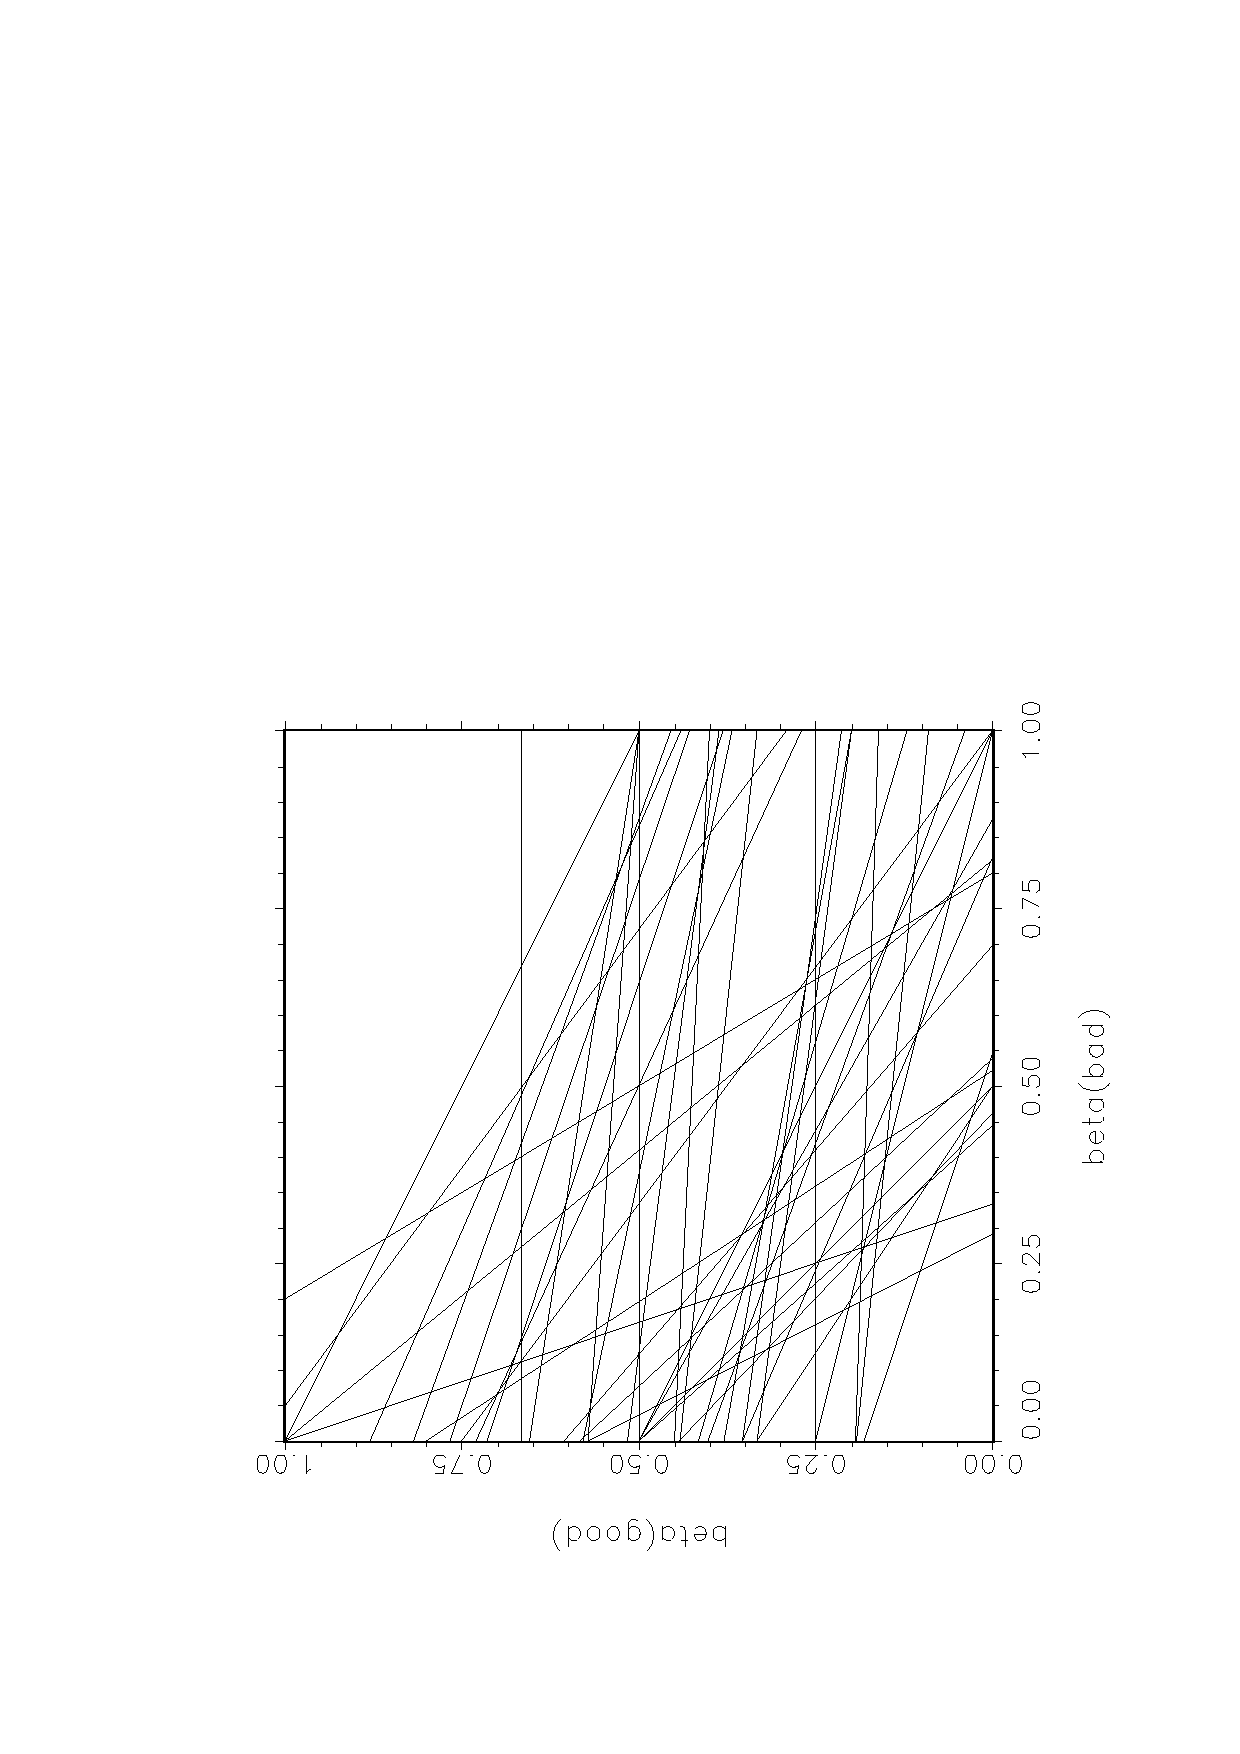
\includegraphics[width=4.5in,height=6in,angle=-90]{tomog}
\caption{\label{fg:tomog}
  Tomography plot for invalid overseas absentee ballots.  $\bb$ and
  $\bg$ are the proportion of Gore's invalid and valid ballots,
  respectively.  Each line traces out the possible values of the
  $\bb_i,\bg_i$ point for each county $i$.}
\end{center} 
\end{figure}

We then add three assumptions, all conditional on $X$ and a set of
covariates $Z$.  First, we assume that $\bb_i$ and $\bg_i$ follow a
truncated bivariate normal distribution, with truncation on the unit
square.  The idea here is that whatever the values of the unknown
parameters from Florida's 67 counties on their respective tomography
lines, they all have something in common, and that any systematic
difference between them will be picked up by covariates.  The main
constraint of this assumption is that the bivariate density is
unimodal.

The second key assumption is that the absence of residual spatial
correlation in $T_i$ after taking into account $X$ and $Z$.  King's
ecological inference model has not been shown to be very sensitive to
anything but extreme levels of spatial autocorrelation, but we make
this assumption even more plausible by including tests with covariates
that tap into Florida's regions and other spatial features

The final assumption states that the two unknown quantities, $\bb_i$
and $\bg_i$, are independent of $X_i$, given $Z$.  For example, if the
\textit{The New York Times} reporters are correct that bad ballots
were cast disproportionately for Bush in Bush counties, then we should
find a strong relationship between $\bb_i$ and variables that measure
Bush support.

\subsubsection{Bayesian Model Averaging}

In Bayesian inference, we are interested in the posterior distribution
which we obtain through the application of Bayes theorem:
\begin{equation}
  \P(\Theta|T) \propto \P(\Theta)\P(T|\Theta).\label{eq:post}
\end{equation}
where $\P(\Theta)$ is the prior probability distribution on some
unknown parameter $\Theta$, and $\P(T|\Theta)$ is the likelihood
(which in our case is given in Equation~\ref{eq:likelihood}).
Everything is conditioned on $X$, $N$, and $Z$, which we observe. We
use the standard independent prior on each parameter of $\Theta$ as
described in section 7.4 of \citet{king:97}.  This prior distribution
and the likelihood function together define King's model in a standard
Bayesian framework.

Along with $T_i$, $X_i$ and $N_i$, we have 25 other variables
including race, sex, and party registration for the overseas absentee
voters as well as county level election and demographic data.  We
define 25 models, each using one of these 25 variables as the
covariate.  We also include a model with no covariates and 3 models
with $X_i$ as the covariate for the mean of $\bb$, $\bg$, and for
both.  For each model, we use the same independent prior distribution
as explained above. The idea of Bayesian model averaging is to produce
one set of results combining these 29 models according to how much
support each model receives from the data.\footnote{A list of all 29
  models follows: (1) no covariate, (2) $X_i$ for $\bb$, (3) $X_i$ for
  $\bg$, (4) $X_i$ for both $\bb$ and $\bg$, (5) military absentee
  voters, (6) registered Republican absentee voters, (7) registered
  Democratic absentee voters, (8) female absentee voters, (9) White
  absentee voters, (10) Black absentee voters, (11) Hispanic absentee
  voters, (12) rejected military absentee voters, (13) rejected
  registered Republican absentee voters, (14) rejected registered
  Democratic absentee voters, (15) rejected female absentee voters,
  (16) rejected White absentee voters, (17) rejected Black absentee
  voters, (18) rejected Hispanic absentee voters, (19) Democratic vote
  share among residents, (20) vote share of other candidates, (21)
  registered Republican residents, (22) registered Democratic
  residents, (23) registered Black Democratic residents, (24)
  registered Black Republican residents, (25) acceptance ratio of
  overall absentee ballots, (26) ratio of invalid absentee ballots,
  (27) Panhandl Florida regional indicator variable, (28) Southern
  Florida regional indicator variable, and (29) corruption indicator
  variable. All the covariates except indicator variables are entered
  as a ratio varying from 0 to 1. Except the first three models, the
  covariate was used to model the conditional untruncted mean of both
  parameters, $\bb$ and $\bg$. For models (5) to (11), each group was
  divided into invalid and valid ballots with the former group used to
  predict $\bb$ and the latter used to predict $\bg$.}

Let $M_k$ denote the $k$th model specification ($k=1,\dots,29$). Then
we make an inference about some quantity of interest $\Delta$ by
computing its posterior distribution via Bayesian model averaging.  To
do this, we first compute, for each of the 29 models, the posterior
distribution of $\Delta$ (computed from Equation \ref{eq:post} with
$\Delta$ being some known function of $\Theta$): $\P(\Delta|M_k,T)$.
Then we average over these models by weighting by the relative
posterior probability that each model is correct, $\Pr(M_k|T)$:
\begin{align} \label{eq:bma}
  \Pr(\Delta|T) &= \sum_{k=1}^{29} \P(\Delta,M_k|T)\notag\\
                &= \sum_{k=1}^{29} \P(\Delta|M_k,T) \Pr(M_k|T)
\end{align}
where the posterior model probability is computed as
\begin{equation}
  \Pr(M_k|T)=\frac{\P(T|M_k)\Pr(M_k)}
             {\sum_{j=1}^{29} \Pr(T|M_j) \Pr(M_j)}.  \label{eq:postmodel}
\end{equation}

To compute the posterior model probability, we need two elements.
First is a prior probability that each model is correct, $\Pr(M_k)$.
For simplicity, we assign an equal prior probability, $1/29$, to each
model.  This at least does not given any a priori advantage to one
model over another.  We conducted sensitivity analyses (reported
below) that did not reveal much change in our overall estimates by
making changes to this prior.

The other quantity we need to compute for the posterior model
probability is the marginal likelihood, $\P(T|M_k)$, which is
\begin{equation}
  \P(T|M_k) = \int \P(T|\Theta_k, M_k) \P(\Theta_k|M_k) d\Theta_k. 
  \label{eq:marglik}
\end{equation} 
where $\P(\Theta_j|M_j)$ is the prior distribution for the parameters
$\Theta$ in Model $k$. That is, the marginal likelihood is obtained by
averaging the likelihood over the prior distribution.  The marginal
likelihood can be thought of as ``the probability of seeing the data
that actually were observed, calculated \emph{before} any data became
available'' \cite[p.776]{kass:raft:95}.  That is, the marginal
likelihood is exactly a likelihood but for the model rather than a
parameter of the model.  Hence, the marginal likelihood tells us how
well each model is supported by the data, just as the likelihood tells
us how well each parameter is supported by a likelihood in traditional
likelihood models.  It is used to calculate the posterior model
probabilities.

\subsection{Estimation and Computational Issues}

The difficulty involved in implementing Bayesian model averaging is
the computation of the marginal likelihood. The integration in
equation~\ref{eq:marglik} is difficult, especially when the prior
distribution on parameters is relatively flat. A number of estimators
have been proposed to improve the precision of the estimation of the
marginal likelihood (see \citet{kass:raft:95} for a comprehensive
survey).

To compute the marginal likelihood, we use the Laplace-Metropolis
estimator, which is based on the idea of combining the asymptotic
approximation and the posterior simulation. This estimator is known to
perform relatively well compared with other methods in many situations
\citep{raft:96,lewi:raft:97,dici:kass:raft:wass:97}.\footnote{If a
  model is estimated through a Markov chain Monte Carlo (MCMC)
  simulation, one can construct an algorithm where the chain visits
  each model stochastically so that you can compute the posterior
  model probability as a direct output of the MCMC posterior draws.
  For example, see \citet{carl:chib:95} and \citet{geor:mccu:93}.
  However, this requires constructing a new MCMC algorithm for each
  application which is not trivial in most situations.  The
  Laplace-Metropolis estimator which we use approximates the marginal
  likelihood without requiring such an effort.  The rate of
  approximation is $O(n^{-1})$, which is considerably better than
  easier-to-apply methods such as BIC, which has a rate of only
  $O(n^{-1/2})$ (see e.g. \citet{kass:tier:kada:89}). For example,
  Kass and Raftery (1995,p.778) say that ``even for very large
  samples, it [BIC] does not produce the correct value.''  In our
  small-$n$ application, the Laplace approximation along with exact
  finite sample posterior simulation is more appropriate.}

% The Laplace-Metropolis estimator of the
% marginal likelihood is based on the following Laplace asymptotic
% approximation.
% \begin{equation}
% \P(T|M_k) \approx (2 \pi)^{d/2}|\widetilde{\Psi}_k|^{1/2}
% \P(T|\widetilde{\Theta}_k) \P(\widetilde{\Theta}_k).
% \end{equation}
% where $\widetilde{\Theta}_k$ is the posterior mode of the objective
% function $f(\Theta_k)=\text{log}(p(T|\Theta_k)p(\Theta))$ and
% $\widetilde{\Psi}_k$ is minus the inverse Hessian of $f(\Theta_k)$
% evaluated at $\Theta_k=\widetilde{\Theta}_k$ for Model $k$. We
% estimate $\widetilde{\Theta}_k$ by taking the values of $\Theta_k$ as
% posterior draws which maximize the objective function.

\section{Empirical Results}
\label{s:outcome}

\subsection{The Probability That Gore Would Have Won Without Bad 
Absentee Ballots}

Figure \ref{fg:margin} portrays the posterior distribution from our
analysis of the Bush's margin of victory if the bad ballots had not
been counted (the histogram of 1000 draws from the posterior).  Note
first that all area for this distribution is contained with the bounds
we found for this quantity of $-119$ to 911.  The weight of the
statistical evidence within these bounds clearly demonstrates that
Bush benefited considerably by the bad ballots, and removing them thus
takes away from his margin.  This is evident in the figure because
almost all of the area of the histogram of posterior probability falls
to the left of the official margin of 537.  The mean margin of victory
for Bush without the bad ballots is only 251 votes.  The figure also
portrays the probability that Gore actually won the election by the
area under the curve to the left of zero.  This is only about 0.2
percent, indicating that Gore probably would not have won, even if the
bad ballots had been discarded.
\begin{figure}[t]
\begin{center}
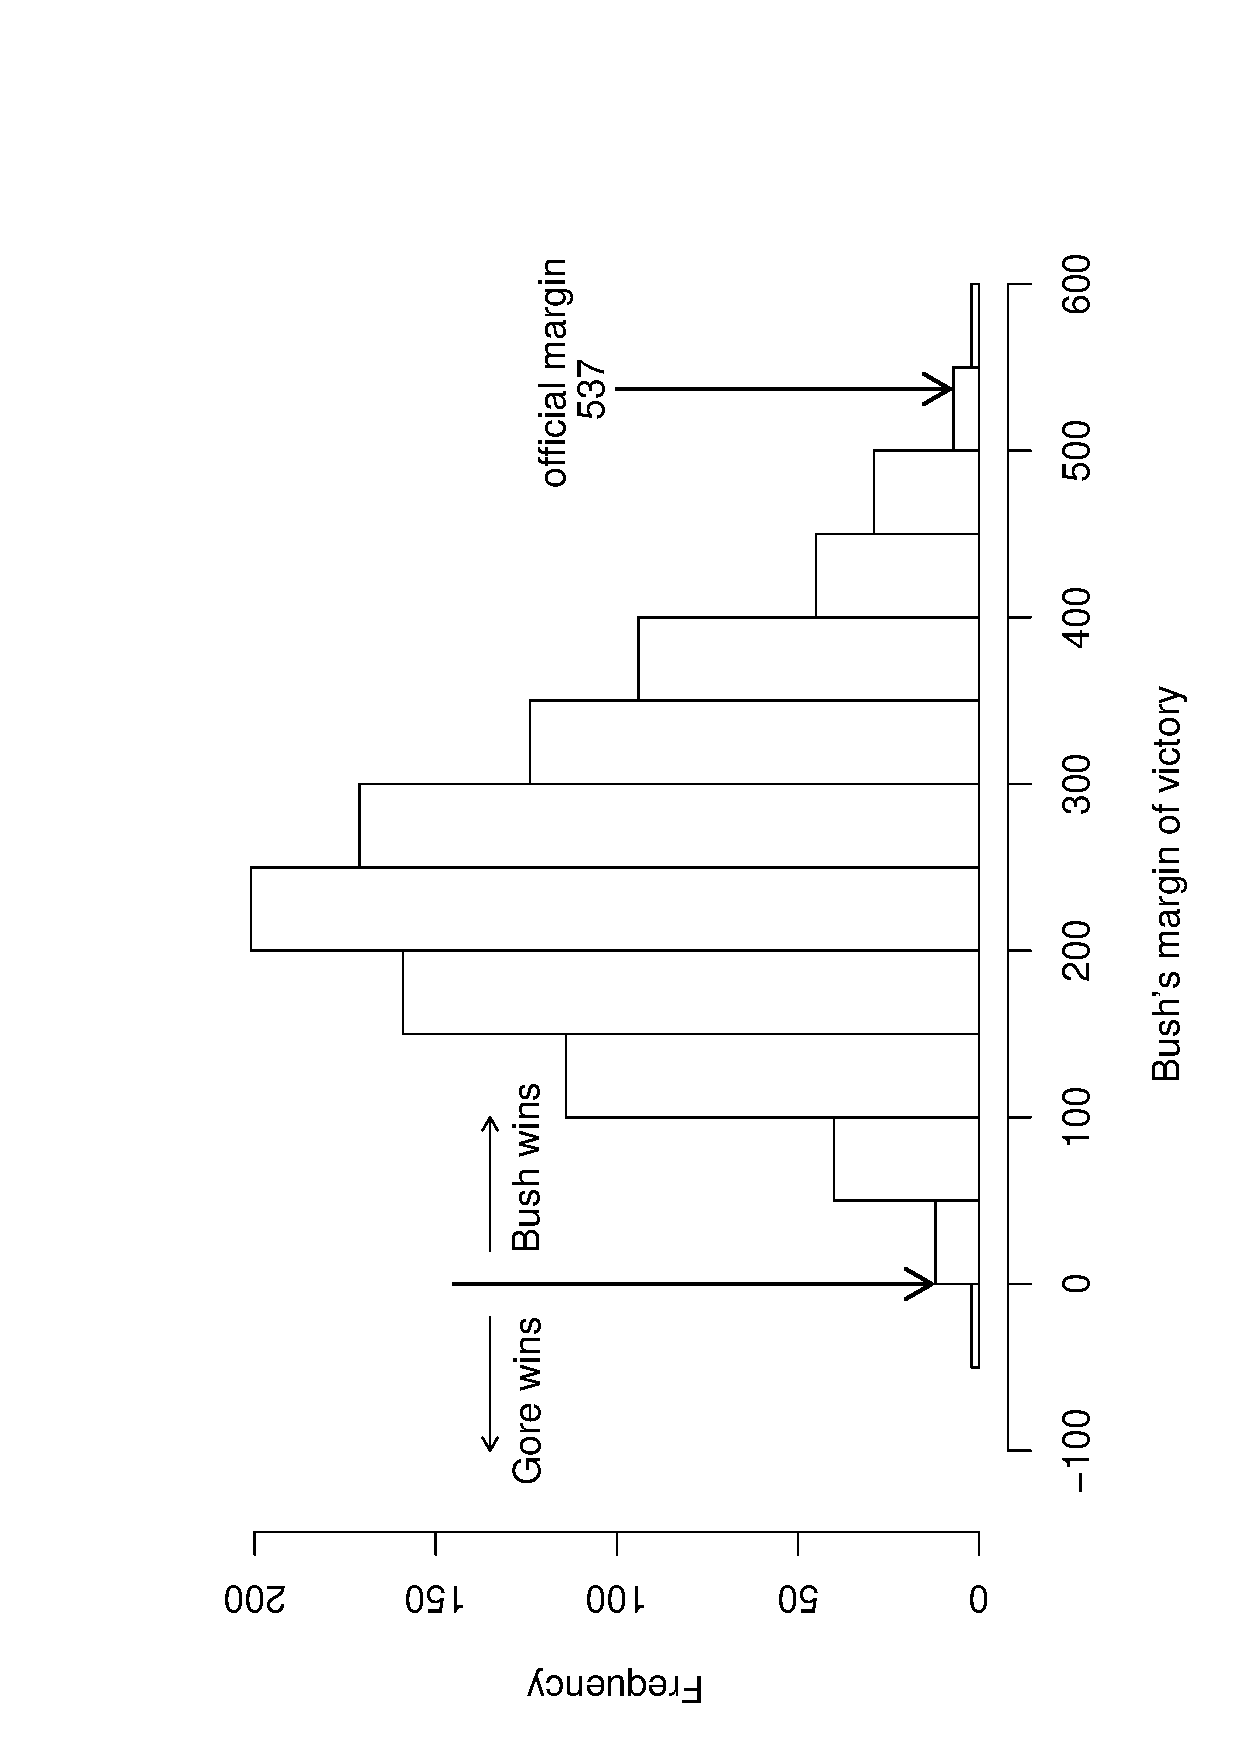
\includegraphics[width=3in,height=4.5in,angle=-90]{margin}
\caption{Posterior distribution of Bush's margin of victory without the
  680 invalid overseas absentee ballots} \label{fg:margin}
\end{center} 
\end{figure}

\subsection{Other Counterfactuals}

While our results indicate that it is unlikely that invalid overseas
absentee ballots alone would have changed the election outcome, the
illegally counted ballots could have had a much more a significant
effect when combined with slight changes in decisions regarding the
manual recounts.  We show this result by first focusing on several
scenarios about the two key counties where a manual recount was
conducted, Miami Dade and Palm Beach. In Miami Dade County, election
officials decided to stop the manual recount when they made the
judgment that they could not meet the recount deadline, set by the
Florida Supreme Court, 5p.m.  Sunday, November 27.  The partial manual
recount gave a net gain of 157 votes to Gore. In Palm Beach county,
they also could not finish the manual recount, but they
submitted the result of the partial recount just before the deadline,
which would have given Gore a net gain of 192 votes for
Gore. Later that day, Palm Beach
electoral officials reported the result of the complete recount to
Harris.  She rejected this complete recount as well as the
partial recount and did not include them in the certified official
tally, thereby denying Gore a total of 349 votes.
\begin{table}[t]
\begin{center}
\begin{tabular}{l..}
 & \multicolumn{1}{c}{Bush's margin} & \multicolumn{1}{c}{Prob(Gore Wins)}\\
\hline
Invalid overseas ballots alone & 251  & 0.002 \\
\emph{Actual recounts}\\
\hspace{1em} Miami Dade partial recount     &  94  & 0.19 \\
\hspace{1em} Palm Beach recount             &  59  & 0.29 \\
\hspace{1em} Miami Dade and Palm Beach    & -98  & 0.82 \\
\emph{Media recounts}\\
\hspace{1em} No U.S.\ Supreme Court decision$^a$ & 242  & 0.01\\
\hspace{1em} Gore's request granted$^b$         & -26  & 0.73\\
\hspace{1em} only fully punched ballots$^c$     & -366 & >0.99 \\
\hspace{1em} hanging chads and dimples$^d$      & -358 & >0.99 \\
\hspace{1em} each county's standard$^e$         & -422 & >0.99 \\
\end{tabular}
\caption{Estimated Bush's margin and Gore's probability of victory
  if the invalid overseas absentee ballots had not been counted along
  with selected other counterfactuals.  $^a$Corresponds to what would
  have happened if the U.S. Supreme Court had not stopped the manual
  recount.  $^b$Gore requested that Broward, Miami-Dade, Palm Beach,
  and Voulusia counties be recounted.  $^c$Only fully punched ballots
  were recounted in all counties.  $^d$Recounting all counties using
  the standard that any hanging chad or dimple was counted.  $^e$A
  recount of the entire state, using the standards adopted by each
  county.} \label{tb:senario}
\end{center}
\end{table}

The panel of Table~\ref{tb:senario} marked ``actual recounts''
presents our prediction for Bush's margin and Gore's probability of
victory in situations where the invalid overseas absentee ballots had
been rejected \emph{and} the recounts in one or both of these counties
had been included in the final tally.  For example, if all the
recounted votes in Miami Dade and Palm Beach had all been counted,
Gore would have won with a 0.82 probability, with the uncertainty in
this number coming only from our analysis of the bad overseas absentee
ballots.  If only the Palm Beach votes had been counted, Gore would
have won with 0.29 probability.  To put it another way, the massive
differences in the probabilities from 0.002 to 0.82 for a Gore victory
were all due to the decisions of Katherine Harris.

In the last panel of Table \ref{tb:senario}, we consider
counterfactuals where the invalid overseas absentee ballots had not
been counted and election day voting recounts had occurred in various
ways, as suggested by a study conducted by a consortium of media
organizations (Fessenden and Broder, 2001).  For example, this
analysis shows that if the U.S.\ Supreme Court had not stopped the
recount in \emph{Bush v.\ Gore}, the victor would have changed with
only a 1\% probability.  However, if Gore's formal request that
Broward, Miami Dade, Palm Beach, and Voulusia counties be recounted
had been granted, then he would have been elected with a 73\%
probability.  If the entire state had been recounted, according to
almost any standard for judging the punch cards, Gore would have won
election with a very high probability.

\subsection{Indirect Evidence of Local Election Officials Responding
  to Republican Pressure}

Six months of interviews and archival research on the ground in
Florida and elsewhere led reporters from the \emph{New York Times}
to conclude that, ``the Republicans mounted a legal and public
relations campaign to persuade canvassing boards in Bush strongholds
to waive the state's election laws when counting overseas absentee
ballots.\ldots Their goal was simple: to count the maximum number of
overseas ballots in counties won by Mr.  Bush, particularly those with
a high concentration of military voters, while seeking to disqualify
overseas ballots in counties won by Vice President Al Gore.''  The
\emph{Times} claimed that as a direct result of this pressure,
``canvassing boards in about a dozen Republican-leaning counties had
reconvened for a second round of counting.  In each place,
longstanding election rules were bent and even ignored.  Boards
counted ballots postmarked as many as seven days after the election,
including some from within the United States.  They counted two
ballots sent by fax.  Officials in Santa Rosa County even counted five
ballots that arrived after the Nov.\ 17 deadline.  Again and again,
election officials crossed out the words `REJECTED AS ILLEGAL' that
had been stamped on ballot envelopes.''

If these claims are correct, we ought to be able to find evidence of
them in our data.  We conduct two tests.  In the first, we divide
Florida's counties into three categories --- the six counties
mentioned explicitly in the \emph{Times} story where the Republicans
were pressured officials to count illegal ballots, the four counties
mentioned where local election officials were pressured not
to count the ballots, and the remaining counties which were not
mentioned.  We then compute various statistic for these three
categories and present them for comparison in Table \ref{t:cty}.
(The results in this table were not available to the reporters before
their article appeared and so Table \ref{t:cty} does represent an
independent test.)
\begin{table}[t]
\begin{center}
  \begin{tabular}{l....|.}

& \multicolumn{1}{c}{military} 
& \multicolumn{1}{c}{Republican} 
& \multicolumn{1}{c}{Bad ballot}
& \multicolumn{1}{c}{Bad Ballots} 
\\ 
& \multicolumn{1}{c}{ballots} 
& \multicolumn{1}{c}{vote} 
& \multicolumn{1}{c}{acceptance$^a$}
& \multicolumn{1}{c}{counted for Bush} 
& \multicolumn{1}{c}{all ballots}\\    \hline
    \multicolumn{5}{l}{\bf Republican pressure to count} \\
    \hspace{1em}Collier  & 46.7\% & 65.6\% & 53.7\% & 64.5\% & 60 \\    
    \hspace{1em}Duval    & 83.8 & 57.5 & 62.3 & 67.8 & 637 \\
    \hspace{1em}Escambia & 88.6 & 62.6 & 64.2 & 80.3 & 272 \\         
    \hspace{1em}Okaloosa & 88.9 & 73.7 & 42.0 & 69.4 & 189 \\          
    \hspace{1em}Pasco    & 62.3 & 48.0 & 60.5 & 76.4 & 53 \\                
    \hspace{1em}Santa Rosa & 90.3 & 72.1 & 84.6 & 84.4 & 93 \\
    \hspace{1em}\emph{Average} & \emph{83}.\emph{4} & \emph{60}.\emph{0} & \emph{61}.\emph{5} & \emph{74}.\emph{3} & 1304 \\
\multicolumn{5}{l}{\bf Counties not mentioned by the \emph{Times}$^b$} \\ 
\hspace{1em}\emph{Average} & \emph{67}.\emph{6} & \emph{51}.\emph{8} & \emph{30}.\emph{0} & \emph{71}.\emph{5} & 1751\\
\multicolumn{5}{l}{\bf Republican pressure not to count}\\ 
    \hspace{1em}Alachua    & 46.8 & 39.8 & 12.5 & 54.5 & 77 \\ 
    \hspace{1em}Broward    & 46.9 & 30.9 & 21.8 & 54.3 & 213 \\  
    \hspace{1em}Miami Dade & 44.4 & 46.3 & 11.7 & 57.1 & 306 \\
    \hspace{1em}Palm Beach & 45.3 & 35.3 & 40.7 & 56.2 & 53 \\ 
    \hspace{1em}\emph{Average} & \emph{45}.\emph{6} & \emph{38}.\emph{1} & \emph{17}.\emph{2} & \emph{55}.\emph{4} &  649 \\
    \hline                                                       
  \end{tabular}                                                
  \caption{Counties classified by whether the \emph{New York Times} 
    reported evidence of Republican pressure to count or not count the
    overseas absentee ballots, compared to an average for the
    remaining counties not mentioned.  Averages are weighted by the
    number of ballots. $^a$The percent of bad ballots that arrived
    with local election officials and were included in the official
    count.}
  \label{t:cty}
\end{center}                                                 
\end{table}

The evidence strikingly supports the \emph{Times} account of events.
The first two columns of Table \ref{t:cty} report on the
characteristics of the county, information available to Republican
strategists before they started lobbying.  With the exception of two
counties with very few absentee ballots, the counties identified as
areas where the Republicans focused their efforts to count ballots
were those with large populations of military personnel and Republican
voters.  Similarly, the counties the \emph{Times} identified as
places where Republicans discouraged the ballots from being counted
had consistently fewer military personnel and Republican voters.

The result of the Republican efforts also appears to have been
successful.  A larger fraction of bad ballots were counted in all
counties where Republicans tried to get them counted than the average,
and a smaller fraction than the average were counted in every county
where the Republicans tried to have them not counted.  
The fraction of bad ballots accepted that had been cast for Bush also
supports the same theory: Fewer of the counted bad ballots had been
Bush voters when the Republicans tried not to have ballots counted
than in every county where the Republicans tried to have them counted.

The \emph{Times'} report also helps explain some interesting
variations in this table.  First, we would have expected more Bush
votes among the bad ballots than we found in Duval County because it
had so many military personnel.  However, the \emph{Times} reported
that an election official on the Duval County canvassing board ``held
the line on counting ballots with missing postmarks.''  Similarly,
Pasco County has relatively low numbers of military ballots and a
small Republican vote share.  So we might expect that this county to
have had relatively few of the bad ballots being cast for Bush.
However, the story also described the unusually strong Republican
pressure applied in this county: ```It looks to me like we've got a
lot of pressure here,' Judge Robert P.  Cole, chairman of the Pasco
board, said as he faced a throng of cheering Republicans and more than
a dozen Bush representatives [and no officials from the Gore
campaign].''  Our quantitative results are certainly consistent with
this qualitative evidence.

We also look for indirect evidence of local election officials
succumbing to pressure from Republican Party officials by examining
which component models in the Bayesian model averaging procedure were
found to have the highest posterior probability.  Table~\ref{tb:bma}
gives the top six such models listed in order.  Generally, if the
\emph{Times'} hypothesis is right, we would expect that the covariates
that have the biggest effects would be related to where
Republicans tried hardest to influence local officials.  If they were
as rational and deliberate as the \emph{Times} indicated, these would
be counties where they expected the largest numbers of bad ballots
that, if counted, would help Bush's cause.  Obviously, we have no such
variable, but there are a variety of variables related to this.  In
the top six, two have the largest effects and both are consistent with
the theory: The more absentee voters registered as Republicans, and the
more white absentee voters in a district, the more bad ballots
were cast for Bush (the negative sign indicating that Bush's lead is
reduced when these ballots are not counted).  The other covariates
have comparatively small effects.
\begin{table}[t]
\begin{center}
\begin{tabular}{l c r@{, }l d{3} d{-3}}
  & \multicolumn{3}{c}{Bush's margin}& \multicolumn{1}{c}{first} 
  & \multicolumn{1}{c}{Posterior model} \\
  & \multicolumn{3}{c}{(95 \% C.I.)} & \multicolumn{1}{c}{difference} 
  & \multicolumn{1}{c}{probability} \\
\hline
Bayesian Model Averaging  & 251 & (69 & 468) & \\
\emph{Individual models}  \\ 
\hspace{1em} Registered Republican absentee voters & 269 & (97 & 475) & $-52$ &  0.565 \\
\hspace{1em} Democratic vote share among residents & 232 & (69 & 448) & 3 &  0.239 \\
\hspace{1em} Black absentee voters                 & 231 & (69 & 440) & $-2$ &  0.102 \\
\hspace{1em} White absentee voters               & 123 & ($-$18& 315) & $-23$ &  0.033 \\
\hspace{1em} Black registered Republican residents & 229 & (62 & 441) & $-6$ &  0.021 \\
\hspace{1em} Accepted absentee ballots             & 218 & (62 & 409) & 4 &  0.004 \\
\end{tabular}
\caption{Estimates of Bush's margin of victory after dropping the
  invalid overseas absentee ballots --- overall and for the six
  component models with the highest posterior model probabilities
  among the 29 models estimated. Each model is identified in the table
  by listing the covariate we used.  The first differences represent
  the increase or decrease in the estimated Bush's margin when the
  value of the covariate is increased by 10 percentage points.}
\label{tb:bma}
\end{center}
\end{table}

Finally, the large variation in our prediction for Bush's margin
across the six models in Table~\ref{tb:bma} emphasizes a clear
advantage of our Bayesian model averaging procedure.  The variation
results from the large degree of model dependence in these data,
largely because the data have fairly wide bounds.  For example, the
specification with white absentee voters gives a confidence interval
which, when considered in isolation from the other models, would not
enable us to reject the hypothesis that Gore won if only the overseas
absentee ballots had been rejected.  This is obviously quite different
from our overall result of only a 0.2 percent probability that Gore
won.  Since different specifications yield very different inferences,
an analyst having to choose one model would be in the untenable
position of having to defend choices without a lot of prior evidence.
Bayesian model averaging offers a way around this common problem.

\subsection{The Minor Effects of Minor Candidates and Prior Densities}

Finally, we analyze the effects of ignoring the minor party candidates
on our results and also study the sensitivity of our results to our
choices for model priors.  Figure~\ref{fg:sensitivity} plots the
posterior distribution of Bush's new margin without invalid overseas
absentee ballots for different model specifications against our
posterior distribution.  The solid line in this figure is an
alternative specification of the ecological inference model where we
combine the votes for the minor candidates together with those for
Gore rather than with the votes for Bush. The posterior distribution
for this model is very similar to the results of our previous analysis
indicating that our results do not depend on which model specification
is used.
\begin{figure}[t]
\begin{center}
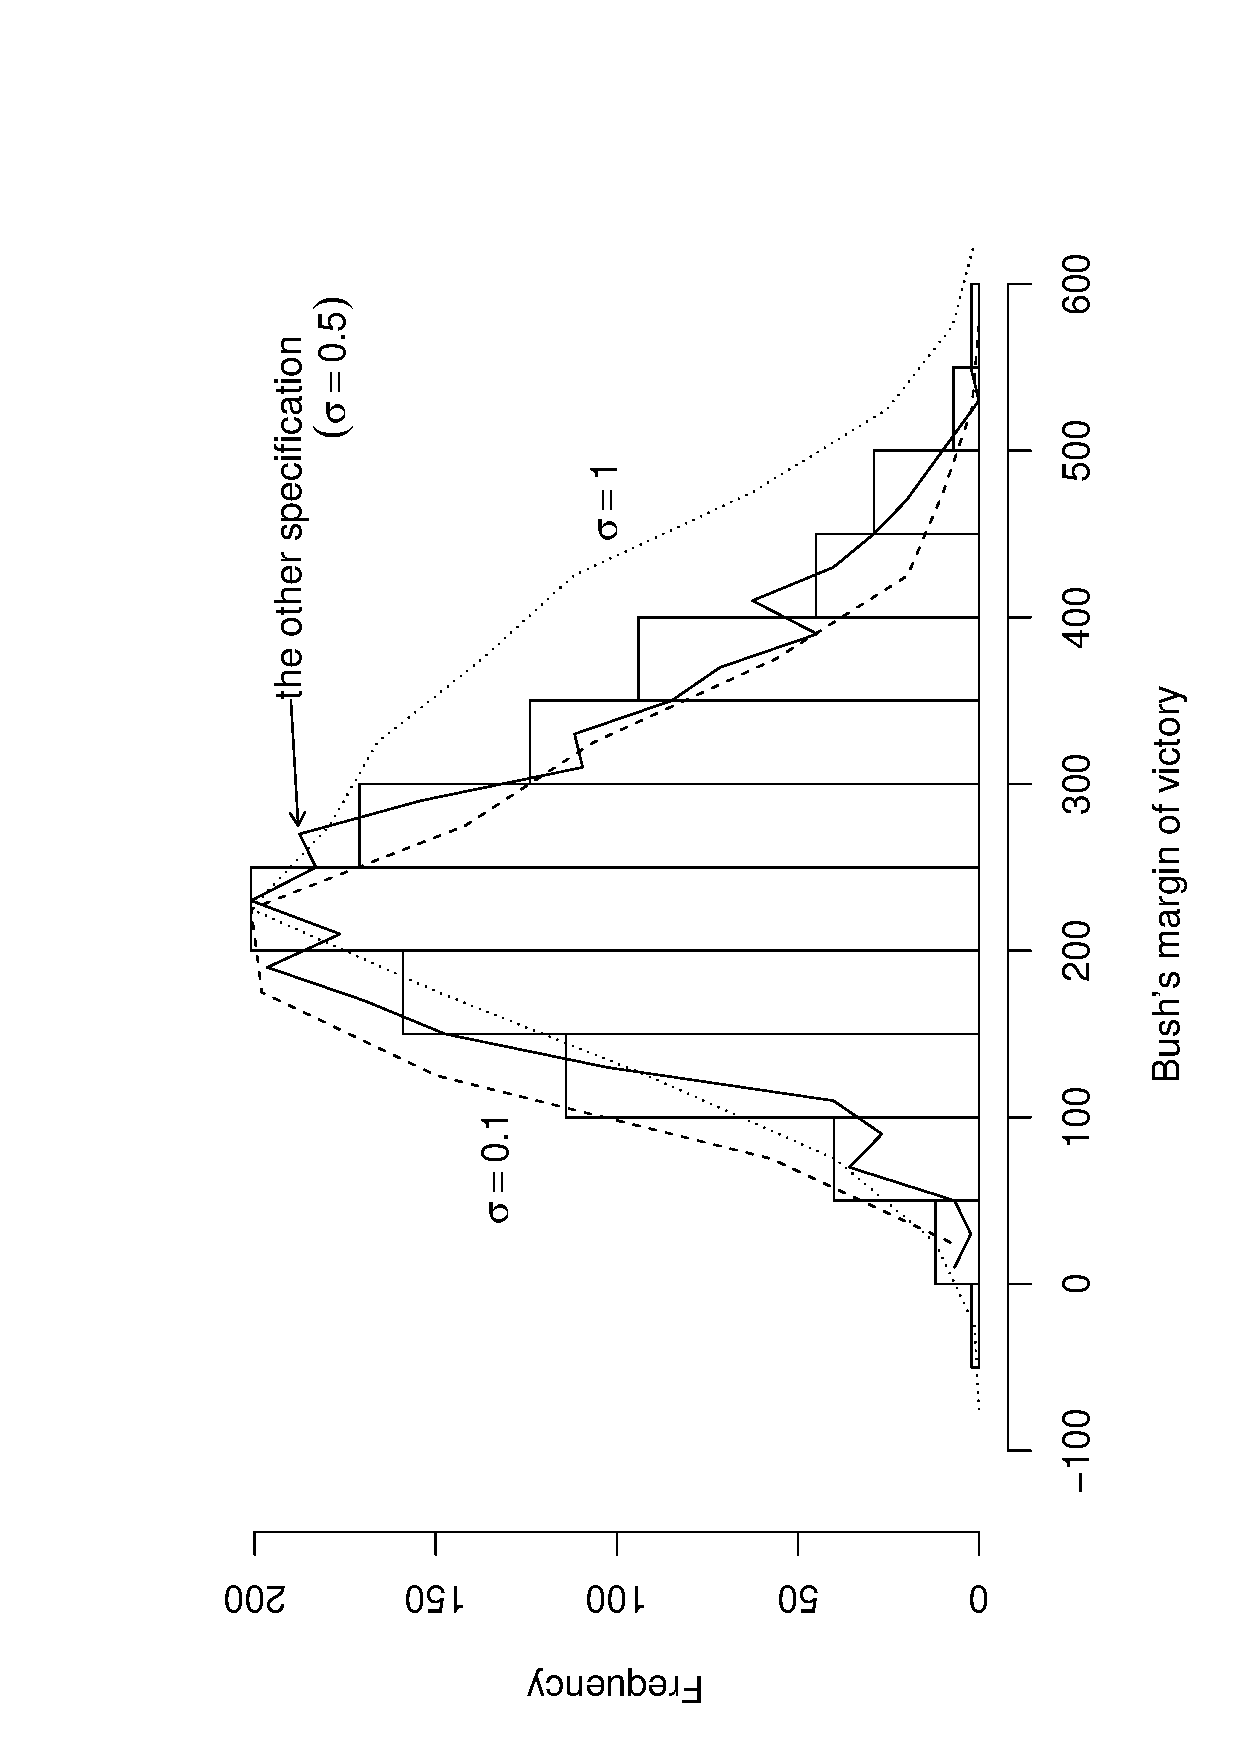
\includegraphics[width=3in,height=4.5in,angle=-90]{sensitivity}
\caption{Sensitivity analysis of Bayesian model
  averaging. The histogram is the posterior distribution of Bush's new
  margin for our model, while the other lines give posterior
  distributions from different models and prior specifications.}
\label{fg:sensitivity}
\end{center} 
\end{figure}

The other two lines represent the use of different prior distributions
for the coefficients of the covariate of each model.  We use different
prior standard deviations for the coefficients of the covariates to
see if the results are sensitive to the choice of the prior
distribution.  While there exists some variation, the graph shows that
the results are not particularly sensitive to the prior specification.

\section{Concluding Remarks}\label{s:concl}

Counterfactual analysis is normally very difficult, and especially so
when the subject of the inference is far from the factual evidence.
When the counterfactual is very close to the data, however, we stand
an especially good chance of making valid inferences (King and Zeng,
2001; Lebow, 2000)\nocite{KinZen01,Lebow00}.  The counterfactuals in
the case of Florida are especially clear and easily could have
happened.  If the problem of the overseas absentee ballots had been
litigated and the law applied equally in every county (as \emph{Bush
  v.\ Gore} seemed to require for votes cast on election day), the bad
ballots might very well have been disqualified.  In this situation,
although Gore probably would have lost, we conclude that no one will
ever be able to say with certainty who would have won the American
presidential election if all American laws had been followed.  If
alsoi the Florida Secretary of State had somewhat different views on
issues that were at least somewhat open to discretion, the outcome of
the election might very well have changed.  Of course, a few different
decisions by the candidates on visits to Florida, campaign spending,
Elian Gonzolas, or any of a variety of other issues might also have
produced a different outcome.

Our results also provide strong, independent, but indirect support for
the \emph{New York Times} thesis that local election officials bent to
the persuasive efforts of Republican strategists to follow the law in
Gore counties and break it in Bush areas.

Finally, we think this paper also provides an especially good example
of the use of Bayesian model averaging.  We have developed the
application of it to the ecological inference model and offer computer
code for others to use it.  In applied work, Bayesian model averaging
has been approximated, such as with the BIC, but its full version has
not seen as much use as it could.

Bayesian model averaging is a clear improvement on the usual situation
of having to select and defend a single model, but it is of course not
a panecia. A researcher never knows whether all relevant models have
been included.  In the present case, where 100\% confidence intervals
are available, we also have some maximum constraints on possible results.

\appendix
\section{A Formal Presentation of the King's Model} \label{appx:king}

The joint distribution of $\bg$ and $\bb$ are assumed to be a
truncated bivariate normal with mean, $\bbetau$, and a variance
$\Sigmau$:
\begin{eqnarray}
\P(\bb_i, \bg_i | \bbetau, \Sigmau) & = & 
\TN (\bb_i,\bg_i | \bbetau, \Sigmau) \\
& = & \N (\bb_i, \bg_i | \bbetau, \Sigmau)
\frac{\mathbf{1}(\bb_i, \bg_i \in [0,1])}
{R(\bbetau, \Sigmau)}.
\end{eqnarray}
where $\mathbf{1}$ is the indicator function, $\N (\bb_i,
\bg_i | \bbetau, \Sigmau) = (2 \pi)^{-1/2} |\Sigmau|^{-1/2}
\text{exp} \{ - \frac{1}{2} (\beta_i-\bbetau)^T \Sigmau^{-1} (\beta_i
- \bbetau) \}$, and $R (\bbetau, \Sigmau) = \int_0^1 \int_0^1 \N
(\bb, \bg | \bbetau, \Sigmau) d\bb
d\bg$.

This distributional assumption together with the account identity
implies the model for the observed data, $T_i$. The resulting
likelihood is the product of a factor, $S(\bbetau, \Sigmau)$, and the
truncated normal density for $\P(\bb_i, \bg_i)$ with
mean, $\Eu(T_i|X_i) = \mu_i = \bbeta^{bad} X_i + \bbetau^g (1-X_i)$
and variance $\Vu(T_i|X_i) = \sigma^2_i$ quadratic in $X_i$, both of
which are on the untruncated scale. Note that $\bbetau=(\bb_i,
\bg_i)$ is a mean vector for the joint distribution,
$p(\bb_i, \bg_i)$. Thus,
\begin{equation}
\P(\Theta|T) \propto \prod_{i=1}^{67} N(T_i|\mu_i, \sigma_i^2)
\frac{S(\bbetau, \Sigmau)}{R(\bbetau, \Sigmau)}. \label{eq:likelihood}
\end{equation} 
where $\Theta$ is the set of all the parameters, $\sigma_i^2=\sigmau_g
+ 2(\sigmau_{bg} - 2 \sigmau_g^2) X_i + (\sigmau_b^2 + \sigmau_g^2 -
2\sigmau_{bg}) X_i^2$ and 
$$S(\bbetau, \Sigmau)=\int_{(\text{max}(0, T_i/X_i-(1-X_i)/X_i),
  \text{min}(1,T_i/X_i))} \N(\bb|\bbetau^b + \omega_i
\epsilon_i / \sigma_i, \sigmau^2_b-\omega^2/\sigma^2_i).$$
Further
details on the derivation of this likelihood function is provided in
King \citeyear[Ch.\ 7]{king:97}.

We control for a vector of covariates $Z_i$ via King's extended model
\cite[Ch.\ 9]{king:97}.  This allows the mean (on the untruncated
scale) of the two unknown parameters $(\bb_i, \bg_i)$ to be a function
of these covariates:
\begin{eqnarray}
\bbetau_i^b & = & [\phi_1 (\sigmau^2_b + 0.25) + 0.5] + (Z_i^b -
\bar{Z}_i^b) \alpha^b \\
\bbetau_i^g & = & [\phi_1 (\sigmau^2_g + 0.25) + 0.5] + (Z_i^g -
\bar{Z}_i^g) \alpha^g
\end{eqnarray}
where $\bbetau_i^b$ and $\bbetau_i^g$ are the conditional means of the
bivariate truncated distribution of $\bb_i$ and $\bg_i$.  This
extension of the model relaxes the assumptions of mean independence,
$E(\bb_i|X_i)=E(\bb_i)$ and $E(\bg_i|X_i)=E(\bg_i)$, and replaces them
with assumptions of conditional independence given the two sets of
covariates $Z_i^b$ and $Z_i^g$.  This also allows for the possibility
of including $X_i$ as a covariate, which is not possible in prior
approaches. 

We specify the prior distribution $p(\alpha^b, \alpha^g, \sigmau^2_b,
\sigmau^2_g, \phi_1, \phi_2, \phi_5)$, where
$\phi_1=(\bbetau^b-0.5)/(\sigmau_b^2+0.25),
\phi_2=(\bbetau^g-0.5)/(\sigmau_g^2+0.25), \phi_5=0.5
\text{ln}\{(1+\rho)/(1-\rho)\}$. This density in turn imply priors on
$\Theta=(\alpha^b, \alpha^g, \phi_1, \phi_2,
\phi_3=\text{ln}\sigmau_b, \phi_4=\text{ln}\sigmau_g, \phi_5)$.  Our
prior specification follows the recommendation of King
\citeyear[chapter7]{king:97}.

\newpage
\singlespacing
\bibliographystyle{/home/willow/king/texinputs/pa}
% \bibliography{/home/who/kimai/localtexmf/BibTeX/stat,/home/who/kimai/localtexmf/BibTeX/polisci}
\bibliography{stat,polisci}

\end{document}
